% !TeX program = pdflatex
% Part B report using the supplied Part A visual system.
\documentclass[12pt,letterpaper]{article}
% ECSE 429 adaptation of the ECSE 211 Profile 1 visual system.
\usepackage{iftex}
\ifPDFTeX
  \usepackage[T1]{fontenc}
  \usepackage{tgtermes}
\else
  \usepackage[no-math]{fontspec}
  % Use installed Times New Roman, with the TeX-distributed equivalent as fallback.
  \IfFontExistsTF{Times New Roman}{\setmainfont{Times New Roman}}%
    {\setmainfont{TeX Gyre Termes}}
\fi
\usepackage[letterpaper,margin=.8in]{geometry}
\usepackage{xcolor,graphicx,amsmath,newtxmath}
\SetSymbolFont{operators}{normal}{OT1}{ntxtlf}{m}{n}
\SetSymbolFont{operators}{bold}{OT1}{ntxtlf}{b}{n}
\SetMathAlphabet{\mathrm}{normal}{OT1}{ntxtlf}{m}{n}
\usepackage{tikz}
\usetikzlibrary{arrows.meta,shapes.geometric,positioning,calc}
\usepackage{array,booktabs,tabularx,enumitem}
\usepackage{caption,fancyhdr,listings}
\usepackage{xurl}
\definecolor{Heading}{RGB}{31,42,60}
\definecolor{Rule}{RGB}{154,167,189}
\definecolor{Caption}{RGB}{90,107,133}
\definecolor{DiagramBlue}{RGB}{49,77,121}
\definecolor{DiagramFill}{RGB}{240,243,247}
\usepackage[unicode,colorlinks=true,linkcolor=Heading,urlcolor=Heading,
  citecolor=Heading,filecolor=Heading,runcolor=Heading,
  pdfdisplaydoctitle=true]{hyperref}
\hypersetup{
  pdftitle={ECSE 429 -- Project Part B Report},
  pdfauthor={James Helou; Jeffrey Lim; Mahan Maalekian; Matthew Petruzziello},
  pdfsubject={Group 3 -- story testing of the Todo Manager REST API}}

\newcommand{\BodyFont}{\fontsize{12bp}{13.8bp}\selectfont}
\newcommand{\TableFont}{\fontsize{10.5bp}{12.2bp}\selectfont}
% Keep headings with their next paragraph without an extra package dependency.
\newcommand{\Needspace}[1]{%
  \par\begingroup\dimen0=#1\relax
  \dimen2=\pagegoal\advance\dimen2 by -\pagetotal
  \ifdim\dimen2<\dimen0\newpage\fi\endgroup}
\setlength{\parindent}{0pt}
\setlength{\parskip}{4bp}
\setlength{\topskip}{0pt}
\setlength{\emergencystretch}{1em}
\raggedright
\AtBeginDocument{\BodyFont}
\pagestyle{fancy}
\fancyhf{}
\renewcommand{\headrulewidth}{0pt}
\renewcommand{\footrulewidth}{0pt}
\fancyfoot[L]{\fontsize{9bp}{11bp}\selectfont\color{Caption}ECSE 429 \quad Group 3}
\fancyfoot[R]{\fontsize{9bp}{11bp}\selectfont\color{Caption}\thepage}

% Retain the ECSE 211 cover's centred blocks and measured baselines.
\newcommand{\CoverLine}[3]{%
  \node[anchor=base,inner sep=0pt,font=\fontsize{#2bp}{#2bp}\selectfont]
    at ([yshift=-#1bp]current page.north) {#3};}
\newcommand{\ReportCover}{%
  \thispagestyle{empty}
  \begin{tikzpicture}[remember picture,overlay]
    \CoverLine{100.14}{16}{\textbf{McGill University}}
    \CoverLine{114.8}{12}{Department of Electrical and Computer Engineering}
    \CoverLine{128.6}{12}{\CourseTitle}
    \CoverLine{212.53}{28}{\textbf{\ProjectTitle}}
    \CoverLine{233.52}{16}{\ProjectSubtitle}
    \CoverLine{254.5}{12}{Report}
    \draw[Rule,line width=.3bp]
      ([xshift=57.6bp,yshift=-271.5bp]current page.north west)
      -- ([xshift=-57.6bp,yshift=-271.5bp]current page.north east);
    \CoverLine{310.65}{14}{\textbf{Group \GroupNumber}}
    \node[anchor=north,inner sep=0pt] at
      ([yshift=-329.68bp]current page.north) {%
      \begin{tabular}{@{}l@{\hspace{1.8em}}r@{}}
        \TeamRoster
      \end{tabular}};
    \CoverLine{472.47}{12}{Prepared \SubmissionDate}
  \end{tikzpicture}
  \null\newpage}

\newcommand{\ReportSection}[1]{%
  \par\Needspace{55bp}\addvspace{6bp}
  {\color{Heading}\fontsize{16bp}{18.4bp}\selectfont\bfseries
   \rule{0pt}{14.94bp}%
   \rlap{\raisebox{-8.26bp}[0pt][0pt]{\color{Rule}\rule{\linewidth}{.3bp}}}%
   #1\par}
  \nobreak\vspace{-2bp}\hrule width 0pt height .3bp
  \nobreak\vspace{5bp}}
\newcommand{\ReportSubsection}[1]{%
  \par\Needspace{40bp}\addvspace{5bp}
  {\color{Heading}\fontsize{13bp}{15bp}\selectfont\bfseries
   \rule{0pt}{12.14bp}#1\par}
  \nobreak\vspace{1bp}}
\newcommand{\RunIn}[1]{\textbf{#1:}\ }
\newcommand{\NewContentPage}{\newpage\BodyFont}
\newcommand{\Path}[1]{\texttt{\fontsize{10.5bp}{12.2bp}\selectfont\detokenize{#1}}}
\newcolumntype{Y}{>{\raggedright\arraybackslash}X}
\newcolumntype{P}[1]{>{\raggedright\arraybackslash}p{#1}}
\newenvironment{ReportTable}[1]{%
  \par\begingroup\TableFont
  \setlength{\tabcolsep}{5bp}\renewcommand{\arraystretch}{1.16}
  \tabularx{\linewidth}{#1}%
}{\endtabularx\par\endgroup\vspace{2bp}}
\newenvironment{Charter}{%
  \par\begingroup\setlength{\leftskip}{12bp}\setlength{\rightskip}{12bp}
  \color{Heading}\itshape
}{\par\endgroup}

\DeclareCaptionFont{captionblue}{\color{Caption}}
\captionsetup[figure]{hypcap=false,font={small,captionblue},labelfont=bf,textfont=normalfont,
  labelsep=period,justification=centering,skip=5bp}
% Styles available for the later diagram-authoring pass.
\tikzset{
  process/.style={draw=DiagramBlue,fill=DiagramFill,line width=.5bp,
    rounded corners=5bp,align=center,inner sep=5bp,
    font=\sffamily\fontsize{9bp}{10.5bp}\selectfont},
  terminal/.style={process,fill=DiagramBlue,text=white},
  decision/.style={diamond,aspect=2.8,draw=DiagramBlue,fill=DiagramFill,
    align=center,inner sep=2bp,font=\sffamily\fontsize{9bp}{10.5bp}\selectfont},
  arrow/.style={-{Stealth[length=4bp,width=3bp]},DiagramBlue,line width=.5bp},
  branch/.style={font=\sffamily\fontsize{8bp}{9bp}\selectfont,text=black}
}
\lstset{
  basicstyle=\ttfamily\fontsize{9.5bp}{11.5bp}\selectfont,
  columns=fullflexible,keepspaces=true,breaklines=true,
  frame=single,framerule=.35bp,rulecolor=\color{Rule},
  backgroundcolor=\color{DiagramFill},framesep=6bp,
  aboveskip=5bp,belowskip=6bp,showstringspaces=false,
  xleftmargin=7bp,xrightmargin=7bp}

\graphicspath{{figures/}}

\newcommand{\CourseTitle}{ECSE 429: Software Validation}
\newcommand{\ProjectTitle}{Project Part B}
\newcommand{\ProjectSubtitle}{Story Testing of REST API}
\newcommand{\SubmissionDate}{November 16, 2026}
\newcommand{\GroupNumber}{3}
\newcommand{\RepoURL}{https://github.com/james-helou/ECSE429-Project-B}
\newcommand{\SourceCommit}{e404151581db239870832037758d61221c01e61a}
\newcommand{\CodeFile}[1]{\href{https://github.com/james-helou/ECSE429-Project-B/blob/e404151581db239870832037758d61221c01e61a/#1}{\Path{#1}}}
% Roster carried over from the team's Part A reference.
\newcommand{\TeamRoster}{%
  James Helou & 261177052\\
  Jeffrey Lim & 261146821\\
  Mahan Maalekian & 261175419\\
  Matthew Petruzziello & 261140144}

\begin{document}
\hypersetup{pageanchor=false}
\ReportCover
\setcounter{page}{1}
\hypersetup{pageanchor=true}
% Target: 5--10 pages. Reflow these manual breaks as final content is added.
% Uppercase placeholders mark the sections Jeffrey will complete.
\ReportSection{1. Summary of Deliverables}
\ReportSubsection{1.1 Project Objective and Scope}
We tested Todo Manager 1.5.5 using stories about how a student organizes coursework
and personal tasks. The API stores todos, projects, categories, and the links
between them. In Part A, we explored these capabilities individually. In Part B,
we used them together to test goals such as recording a task, adding it to a
course project, and checking what work remains.

\begin{ReportTable}{@{}P{.28\linewidth}P{.12\linewidth}Y@{}}
\toprule
\textbf{Measure} & \textbf{Count} & \textbf{Explanation}\\
\midrule
User stories & 20 & Goals covering todos, categories, projects, and their relationships.\\
\textit{Scenario Outlines} & 72 & Normal, alternate, and error flows.\\
Executed examples & 146 & One case for each row in the \textit{Examples} tables.\\
Passed examples & 122 & Cases that met their acceptance criteria.\\
Failed examples & 24 & Cases linked to nine findings in the bug report.\\
Policy-related failures & 16 & A subset of the 24 failures, checking workflow rules the API does not clearly promise.\\
\bottomrule
\end{ReportTable}

\ReportSubsection{1.2 Deliverables}
\begin{ReportTable}{@{}P{.24\linewidth}Y@{}}
\toprule
\textbf{Deliverable} & \textbf{Location and role}\\
\midrule
Written report & Describes the story coverage, test suite, reproduction steps, execution results, and findings.\\
Story test suite & \Path{ECSE429-Project-B/}: feature files, step definitions, shared helpers, setup code, dependency files, and the application JAR.\\
Bug report & \Path{BUG_REPORT.md}: expected and actual behavior, potential impact, reproduction steps, and related story IDs.\\
Execution records & \Path{Verification/}: Cucumber results, console logs, source hashes, and additional API checks. Section~8 lists the files used in this report.\\
\bottomrule
\end{ReportTable}

\ReportSubsection{1.3 Connecting the Tests and Findings}
\begin{center}
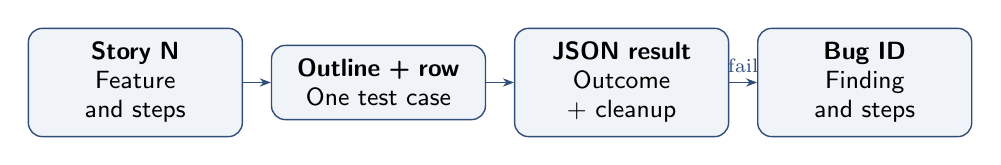
\begin{tikzpicture}[node distance=10bp]
\node[process,text width=.195\linewidth] (story)
{\textbf{Story N}\\Feature and steps};
\node[process,text width=.195\linewidth,right=of story] (example)
{\textbf{Outline + row}\\One test case};
\node[process,text width=.195\linewidth,right=of example] (result)
{\textbf{JSON result}\\Outcome + cleanup};
\node[process,text width=.195\linewidth,right=of result] (finding)
{\textbf{Bug ID}\\Finding and steps};
\draw[arrow] (story)--(example);
\draw[arrow] (example)--(result);
\draw[arrow] (result)--node[above,font=\fontsize{7bp}{8bp}\selectfont]{fail}(finding);
\end{tikzpicture}
\end{center}
Source hashes identify the code used for the run. Bug IDs connect failed cases
to their explanations in \Path{BUG_REPORT.md}.

\ReportSubsection{1.4 Team Participation}
\begin{ReportTable}{@{}P{.25\linewidth}P{.10\linewidth}P{.20\linewidth}Y@{}}
\toprule
\textbf{Member} & \textbf{Stories} & \textbf{Area} & \textbf{Other responsibilities}\\
\midrule
James Helou & 1--5 & Todos & Harness and shared steps\\
Jeffrey Lim & 6--10 & Categories & Written report\\
Mahan Maalekian & 11--15 & Interoperability & Integration and submission ZIP\\
Matthew Petruzziello & 16--20 & Projects & Videos\\
\bottomrule
\end{ReportTable}

\NewContentPage
\ReportSection{2. Story Testing Method}
\ReportSubsection{2.1 User Stories and Acceptance Criteria}
We chose a student organizing coursework and personal tasks as our user. Each
story describes something the student wants to do and why it is useful. For
example, Story 6 states: ``As a student, I want to create a category so that I can
organize my work into meaningful groups.'' The acceptance tests then check
whether the API supports that goal.

We used our Part A findings to decide what to check after each operation.
Relationship tests read the association from both objects, deletion tests check
whether references remain, and write tests read back the stored records. This
matters because a request can return a successful status while leaving the data
in an unexpected state. We compared the results with the API documentation and
the expected behavior recorded in our bug report~[\ref{ref:api},\ref{ref:bugs}].

\ReportSubsection{2.2 Normal, Alternate, and Error Flows}
Every feature has a \textit{Background} and at least one normal, alternate, and error
\textit{Scenario Outline}. The \textit{Background} starts the application and creates the data
needed for each example. The normal flow completes the main operation. The
alternate flow reaches the goal with a different valid input or approach. The
error flow checks what happens when the operation cannot be completed.

For Story 6, the normal flow creates a category with a title and description.
The alternate flow creates one with only a title. The error flow submits an empty
title and expects HTTP 400 with the validation message. It also compares the
stored records before and after the request, because rejecting the input should
leave the system unchanged.

Each \textit{Examples} table supplies the data for its \textit{Scenario Outline}. Most outlines
have two rows, while two todo outlines have a third row. Our 72 outlines therefore
produce 146 cases, including the relationship and filter checks that reproduce
our reported findings.

\ReportSubsection{2.3 Deciding What the API Should Do}
Some expectations follow from the documentation or from the operation itself.
For example, asking for a missing project's tasks should not return work from
another project. Our test accepts either HTTP 404 with the expected error shape
or HTTP 200 with an empty task array, because the documentation does not specify
an exact missing-project response for this query.

Other expectations come from how we want the student workflow to behave. These
include seeing category membership from both objects, accepting a numeric ID
where its string form works, and preserving links when changing only a title.
Where the API does not clearly promise this behavior, we mark the failing
scenario with both \Path{@bug} and \Path{@policy}. This way, the result shows
which expectation failed and whether that expectation is an established API rule
or a rule we chose for the workflow. We treat supported inline creation through
a relationship request as a valid alternate flow.

\NewContentPage
\ReportSection{3. User Stories and Acceptance Coverage}
\ReportSubsection{3.1 Story Coverage}
The table lists the outlines for each story and its example results with seed 765432.
\begin{ReportTable}{@{}P{.05\linewidth}YP{.09\linewidth}P{.08\linewidth}P{.07\linewidth}@{}}
\toprule
\textbf{ID} & \textbf{User goal} & \textbf{Outlines} & \textbf{Pass} & \textbf{Fail}\\
\midrule
1 & Record a task on the todo list & 3 & 7 & 0\\
2 & Mark a task as done & 3 & 7 & 0\\
3 & Change the wording of a task & 3 & 6 & 0\\
4 & Remove a task from the todo list & 3 & 6 & 0\\
5 & See what is left to do & 5 & 6 & 4\\
6 & Create a category & 3 & 6 & 0\\
7 & View category details & 3 & 6 & 0\\
8 & Rename a category & 3 & 6 & 0\\
9 & Edit a category's description & 3 & 6 & 0\\
10 & Delete a category & 3 & 6 & 0\\
11 & Add a task to a course project & 5 & 6 & 4\\
12 & Take a task off a course project & 4 & 6 & 2\\
13 & Tag a task with a category & 5 & 6 & 4\\
14 & File a course project under a category & 5 & 6 & 4\\
15 & See what is left on a course project & 6 & 6 & 6\\
16 & Record a course project & 3 & 6 & 0\\
17 & Correct project details & 3 & 6 & 0\\
18 & Complete or reopen a project & 3 & 6 & 0\\
19 & Remove a project & 3 & 6 & 0\\
20 & Find a course project & 3 & 6 & 0\\
\midrule
 & \textbf{Total} & \textbf{72} & \textbf{122} & \textbf{24}\\
\bottomrule
\end{ReportTable}

\ReportSubsection{3.2 Example of an Acceptance Test}
In Story 6, the \textit{Background} runs for each \textit{Examples} row before the normal, alternate,
or error flow begins. The normal flow checks category creation as follows:
\begin{enumerate}[leftmargin=1.6em,itemsep=2bp,topsep=4bp]
\item Create the initial records and save their state for this example.
\item Read the title and description from the example row: ``Coursework / anything with marks'' or ``Errands / things to do on campus.''
\item Create the category and check for HTTP 201.
\item Read the category back and compare its title and description with the supplied values.
\item Check that exactly one category was added and that unrelated records stayed unchanged.
\end{enumerate}
The alternate flow omits the description, while the error flow supplies an empty
title.

\ReportSubsection{3.3 Coverage Limits}
The suite covers selected student workflows. A finding can affect several
examples or stories, so the failed-example count and the finding count measure
different things.

\NewContentPage
\ReportSection{4. Structure of the Story Test Suite}
\ReportSubsection{4.1 Feature Files and Step Definitions}
Cucumber.js reads the feature files and matches their steps to JavaScript
functions in \Path{steps/}. Each story has its own step-definition file. We put
common fixture setup, response checks, and cleanup in \Path{steps/stepDefs.js}
so that several stories can use the same steps. \Path{TestUtil.js} handles HTTP
requests and record lookups, while Chai assertions check the responses and stored
results.

\begin{center}
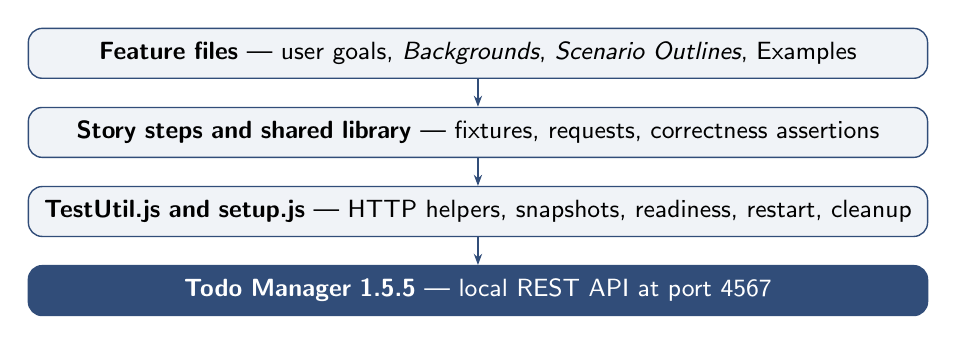
\begin{tikzpicture}[node distance=10bp]
\node[process,text width=\dimexpr\linewidth-30bp\relax] (features)
{\textbf{Feature files} --- user goals, \textit{Backgrounds}, \textit{Scenario Outlines}, Examples};
\node[process,text width=\dimexpr\linewidth-30bp\relax,below=of features] (steps)
{\textbf{Story steps and shared library} --- fixtures, requests, correctness assertions};
\node[process,text width=\dimexpr\linewidth-30bp\relax,below=of steps] (helpers)
{\textbf{TestUtil.js and setup.js} --- HTTP helpers, snapshots, readiness, restart, cleanup};
\node[terminal,text width=\dimexpr\linewidth-30bp\relax,below=of helpers] (api)
{\textbf{Todo Manager 1.5.5} --- local REST API at port 4567};
\draw[arrow] (features)--(steps);
\draw[arrow] (steps)--(helpers);
\draw[arrow] (helpers)--(api);
\end{tikzpicture}
\captionof{figure}{How acceptance scenarios reach the API and assess its behavior.}
\label{fig:architecture}
\end{center}

\ReportSubsection{4.2 Setup, Assertions, and Cleanup}
The shared readiness step stops any existing API instance and starts the bundled
JAR. It waits for HTTP 200 and a todos array, then records the seeded todos,
projects, and categories. The remaining \textit{Background} steps create the fixtures for
the example. Each scenario keeps its responses and selected IDs in Cucumber's
\Path{this} state, which is separate for each case.

After a write, the steps read back the data to check what was stored. Where a
change should affect only one record, the tests also compare the other records
with the saved state. This allows the tests to detect unwanted side effects
that would not be apparent from the response status alone.

The \textit{After} hook runs even if an assertion fails. It stops and restarts the JAR,
compares the seeded records with the initial snapshot, and stops the service
again. Before comparison, the helpers sort records and relationship references
by ID so that a different array order does not cause a false failure.

\ReportSubsection{4.3 Independence and Code Organization}
Each example gets a fresh application process and creates its own fixtures.
Helpers use returned IDs or look up records by title, so the tests do not need
to predict which ID will be allocated next. Shared request and payload functions
keep the HTTP handling in one place. Conversion of Gherkin strings to booleans
is limited to the boolean fields, leaving invalid values intact for error tests.
HTTP requests have a five-second timeout, with separate time limits for readiness
and application startup and shutdown.

\NewContentPage
\ReportSection{5. Source Repository and Reproduction}
\ReportSubsection{5.1 Repository Structure}
Our source repository is
\url{https://github.com/james-helou/ECSE429-Project-B}.
We verified the executable code at commit \Path{e404151}. Later changes to
\Path{README.md} and \Path{BUG_REPORT.md} update the written explanations.
Section~8 gives the full commit ID and the execution records.

\begin{lstlisting}
ECSE429-Project-B/
+-- features/
|   +-- Story<N>*.feature         User stories and examples
+-- steps/
|   +-- Story<N>StepDefs.js       Steps for each story
|   +-- stepDefs.js              Shared steps and After hook
+-- TestUtil.js                  HTTP requests and record checks
+-- setup.js                     API startup, reset, and shutdown
+-- package.json                 Run commands and dependencies
+-- package-lock.json            Locked dependency versions
+-- runTodoManagerRestAPI-1.5.5.jar
+-- BUG_REPORT.md                Findings and reproduction steps
+-- README.md                    Setup and run instructions
\end{lstlisting}

\ReportSubsection{5.2 Environment and Run Instructions}
We ran the November 16 checks on Windows using Microsoft OpenJDK 17.0.12,
Node.js 22.13.1, npm 11.6.2, Cucumber.js 11.3.0, and Chai 4.5.0.
The suite requires Java and Node 18 or newer. From the repository directory,
install the dependencies and run the tests. On our Windows machine, we selected
the installed JDK with the following PowerShell commands:
\begin{lstlisting}
$env:JAVA_HOME = 'C:\Program Files\Microsoft\jdk-17.0.12.7-hotspot'
npm.cmd ci
npm.cmd run cucumber
\end{lstlisting}
The harness starts and stops the JAR automatically. Keep port 4567 free and run
one suite at a time. If an API instance is already answering on that port, the
harness shuts it down and its in-memory data is discarded.

\ReportSubsection{5.3 Changing the Order and Stopping the Service}
The default run uses random seed 765432. The commands below select a different
order and save its results, then run the service-stopped check:
\begin{lstlisting}
npx.cmd --no-install cucumber-js ./features -r ./steps `
  --order random:20261117 --format summary `
  --format json:results-seed-20261117.json
npm.cmd run cucumber:no-server
\end{lstlisting}
For the last command, leave the API stopped. Autostart is disabled, so every case
should fail at the readiness step. We expect exit code 1 because failures are
expected. To run only cases without the
\Path{@bug} tag, use \Path{npm run cucumber:no-bugs}.

\NewContentPage
\ReportSection{6. Findings of Story Test Execution}
\ReportSubsection{6.1 Recorded Results}
We ran the full suite with seed 765432, with 122 of the 146 cases passing and
24 failing. There were 1,051
passed steps, 24 failed steps, and four skipped steps. The skipped steps followed
failed assertions.

\begin{ReportTable}{@{}Yrrr@{}}
\toprule
\textbf{Area / story IDs} & \textbf{Cases} & \textbf{Passed} & \textbf{Failed}\\
\midrule
Todos / 1--5 & 36 & 32 & 4\\
Categories / 6--10 & 30 & 30 & 0\\
Interoperability / 11--15 & 50 & 30 & 20\\
Projects / 16--20 & 30 & 30 & 0\\
\midrule
\textbf{Total} & \textbf{146} & \textbf{122} & \textbf{24}\\
\bottomrule
\end{ReportTable}

All category and project cases passed. The passing cases covered creating,
reading, changing, and deleting records, as well as the ordinary relationship
operations. The failures were concentrated in relationship behavior and todo
filters. These results describe the workflows and data in our suite; other API
routes and input combinations would need their own tests.

\ReportSubsection{6.2 Readiness, Order Independence, and State Restoration}
We repeated the full run with seed 20261117. The seed changed the order of the
tests, but each case produced the same result and each failing case stopped at
the same assertion. Each example starts a fresh application process, creates
its own fixtures through its \textit{Background}, and keeps its responses and IDs
in separate scenario state. Because the cases establish their own starting
conditions, they do not rely on data left by an earlier test. The matching
results across the two orders support this design.


The \textit{After} hooks restored the seeded records and stopped the service after
each case, including those with failed assertions. The restoration checks passed
in both orders, confirming that cleanup completed even when a test failed.

With autostart disabled and the API stopped, every case failed at readiness.
The cleanup hooks still completed successfully. This confirms that the suite
detects an unavailable service before attempting the scenario operations.

\NewContentPage
\ReportSubsection{6.3 Bug Findings and Remaining Risks}
The 24 failed examples relate to the nine findings below. All carry \Path{@bug},
and 16 also carry \Path{@policy}. Each finding describes the expected and actual
behavior, its impact, and the affected stories. The full reproduction steps are
recorded in \Path{BUG_REPORT.md}.

\begin{ReportTable}{@{}P{.09\linewidth}P{.11\linewidth}YP{.06\linewidth}@{}}
\toprule
\textbf{ID} & \textbf{Story} & \textbf{Observed outcome and consequence} & \textbf{Fails}\\
\midrule
BR01 & 15 & Missing/deleted project task reads return unrelated work; students can see tasks outside the selected project. & 4\\
BR03 & 13, 14 & Category membership appears only on the writing side; reverse browsing can hide filed work. Reciprocity is a policy. & 6\\
BR04 & 13 & A deleted category remains readable through a task link after direct GET returns 404. & 2\\
BR06 & 11 & Plain XML IDs return 404 while equivalent CDATA and JSON strings link successfully. & 2\\
BR19 & 11 & Numeric JSON IDs return 404 while string IDs work. Numeric coercion is a policy. & 2\\
BR32 & 15 & Title-only project PUT removes task links. Preserving omitted links is a policy. & 2\\
B-N1 & 12 & Title-only task PUT removes its project link; a rename can lose filing. Preservation is a policy. & 2\\
B-N2 & 5 & Invalid done-status filters return 200 with an empty list. Rejecting them is a policy. & 2\\
B-N3 & 5 & Unknown query fields are ignored and return unfiltered work. Rejecting them is a policy. & 2\\
\bottomrule
\end{ReportTable}

\ReportSubsection{6.4 New Findings and Their Consequences}
\RunIn{B-N1: Title-only task replacement removes its project link}
We created a project with two tasks and sent a PUT containing only a new title
to one task. Reading the project's tasks and the task's reverse \Path{tasksof}
view showed that the selected link had been removed, while the other task
remained. Our workflow expects a wording change to preserve project membership,
but the API does not clearly promise this for PUT. Sending the title change
through POST preserved the link.

\RunIn{B-N2: Invalid done-status filter is accepted}
With unfinished and completed todos present, we compared valid boolean filters
with \Path{doneStatus=maybe} and \Path{doneStatus=not-a-boolean}. The invalid
queries returned HTTP 200 and an empty list. Our chosen rule expects HTTP 400,
because an invalid filter should be distinguishable from having no work left.
The API rejects invalid booleans when creating a todo, but that does not establish
the same validation rule for queries.

\RunIn{B-N3: Unknown todo filter is ignored}
We captured the todo list, then queried \Path{colour=red} and \Path{doneStats=red}.
Both returned the same unfiltered records. A valid title filter returned one
record. Our workflow expects HTTP 400 for unknown fields, although the
documentation does not specify that rule. Ignoring a misspelled field can make
a student think a filter was applied when it was not.

\RunIn{What needs attention}
We would prioritize unrelated project data and references to deleted categories,
because both can cause the student to act on the wrong records. Additional
checks reproduced the XML difference, a deleted category in a project
view, and the unknown-filter results~[\ref{ref:probes}]. BR17 records supported
inline creation in stories 11 and 13.

\NewContentPage
\ReportSection{7. AI Assistance Disclosure}
\ReportSubsection{7.1 AI Tools Used}
We used AI to help with repetitive implementation work and to make our project
documents more concise. We wrote the main user stories, feature files, and
scenario outlines, and chose the behavior we wanted to test. We also wrote the
expected failures in \Path{BUG_REPORT.md}. AI helped us shorten those descriptions
while keeping the expected behavior, observed results, and impact clear.

We wrote JavaScript code for the suite and used AI to help with its
implementation, particularly the helpers and the consistency of code written by
different team members. This included organizing shared steps, applying common
request and assertion patterns, and helping the separate stories work together
in one suite. We used Codex to help set up the LaTeX formatting, format our
writing into paragraphs, tables, and lists, and revise the wording.

\ReportSubsection{7.2 Verification of AI Output}
We ran the suite and compared the results with the expected behavior in our
scenarios and bug report. Running with different random seeds checked whether
the cases behaved consistently when their order changed. The restoration checks
and service-stopped run also checked the setup and cleanup behavior. These checks
helped us assess whether the shared code supported the tests we intended to run.

For the written report, we reviewed the text against our test design and
recorded results. Shorter wording still needs to preserve
what we tested, what we expected, and what actually happened. The LaTeX output
was also compiled and checked for layout issues.

\ReportSubsection{7.3 Strengths and Limitations}
AI helped us apply common patterns across similar tests and reduce repeated
code. This was useful when combining work from several people, because the
stories needed to use the same helpers and behave consistently within the suite.
It also helped us organize the results and express our findings more clearly.

However, AI can misunderstand an expected outcome or suggest an assertion that
checks the wrong thing. A test passing only shows that its assertions were met.
It does not establish that those assertions describe the intended behavior.
The same applies to the report: making an explanation shorter is useful only if
it still matches the scenario and its evidence.

\ReportSubsection{7.4 Prompt Examples}
\begin{enumerate}[leftmargin=1.6em,itemsep=6bp,topsep=4bp]
\item ``Implement this text block ... into the LaTeX and break it up into a numbered list form.''
\item ``In my categories test suite I implemented helpers. I know that in this file it does something similar. Can you abstract it to use the same helper?''
\item ``Can you make the BUG\_REPORT markdown more concise?''
\end{enumerate}

\NewContentPage
\ReportSection{8. References and Supporting Artifacts}
The links below identify the source code used for the tests. The execution
records are stored in \Path{Project/Part2/Verification/}, beside the repository
in our working directory.

\begin{enumerate}[label={[\arabic*]},ref=\arabic*,leftmargin=2em,itemsep=8bp,topsep=6bp]
\item\label{ref:api} Todo Manager 1.5.5 REST API documentation, served while the application is running: \url{http://localhost:4567/docs} and \url{http://localhost:4567/docs/swagger}.
\item\label{ref:source} Group 3. \href{https://github.com/james-helou/ECSE429-Project-B}{ECSE429-Project-B repository}. Tested executable revision:\\
\Path{e404151581db239870832037758d61221c01e61a}.\\
Source organization: \href{https://github.com/james-helou/ECSE429-Project-B/tree/e404151581db239870832037758d61221c01e61a/features}{\Path{features/}}, \href{https://github.com/james-helou/ECSE429-Project-B/tree/e404151581db239870832037758d61221c01e61a/steps}{\Path{steps/}}, \CodeFile{TestUtil.js}, and \CodeFile{setup.js}. The README and bug report contain later documentation edits.
\item\label{ref:bugs} Group 3. \Path{ECSE429-Project-B/BUG_REPORT.md}, November 16 version. Nine failing findings, their policy/contract distinctions, reproduction steps and impact; BR17 records supported inline creation.
\item\label{ref:finalrun} November 16 full-run and outage evidence:\\
\Path{final-check-2026-11-16.json} and \Path{.log};\\
\Path{final-check-2026-11-16-source.json};\\
\Path{final-check-2026-11-16-summary.json} and \Path{.md};\\
\Path{final-outage-2026-11-16.json} and \Path{.log}.
\item\label{ref:orders} Execution-order comparison:\\
\Path{report-final-seed-20261117.json} and \Path{.log}.\\
Earlier November 15 comparison: \Path{repaired-full-seed-765432.json} and \Path{repaired-full-seed-20261117.json}, with their logs and tested-source hashes. The November 16 runs above verify the current executable code.
\item\label{ref:probes} November 16 targeted probes: \Path{bug-report-probes-2026-11-16.json}. Controls compare plain XML, CDATA and JSON; direct versus linked deletion reads; and valid versus unknown filters.
\item\label{ref:assignment} ECSE 429 project specification, Part B (pp.~5--6), with the Part A bug format (p.~4); Fall 2026 course project overview, generative AI disclosure requirements (p.~5).
\end{enumerate}

\ReportSubsection{PUT REFERENCES TO ZIP AND VIDEO HERE}

\end{document}
